%\newpage
  \begin{titlepage}
    \vspace*{\fill}
      \part{Feature detection}
    \vspace*{\fill}
  \end{titlepage}

%\chapter{Feature Detection}\label{ch:feature_detection}
\phantomsection
\chapter*{Contents}

\textit{Before getting to the main part of this project that is Feature extraction, there is a mandatory step that is Feature detection. In order to avoid the more computation and processing as possible, only the parts that contains the regions of interest for a Facial Expression Recognition system have to be processed. It means by consequence that there has to be beforehand the detection of the interesting features. This detection can be summarized into face detection. This part will explain how face detection works in general. Then the most famous and efficient algorithm for face detection will be introduced and studied. This algorithm is the Viola-Jones algorithm.}
\pagebreak

\phantomsection
\chapter{Face detection}

\noindent Face detection is the first step after image acquisition. It represents a requirement for a Facial Expression Recognition system. All the background is not taken into account. It allows to focus only on what is interesting in the input image: the face, which helps reducing the processing during the next step that is feature extraction.
\newline

\phantomsection
\section{Detection}

\vspace{\baselineskip}
\noindent Finding out if the input image or video sequence represents or contains a particular object is what is called Detection. Usually after the detection step comes the recognition step. For this system, the recognition step consists in facial expression recognition. But depending on the recognition, there can be another step that is the tracking step. Tracking consists in following a moving target on the images of a video sequence \cite{DIN08}.
\newline

\noindent To represent an object detector, the term "black box" can be used. The box gets an image as its input and at a high level the output can be considered as an image with annotations saying where the object of interest appears, if it appears \cite{DIN08}. For example, the output can look like in figure~\ref{output_example_face_detection} \cite{DIN08}.
\newline

\begin{figure}[!h]
\begin{center}
\noindent 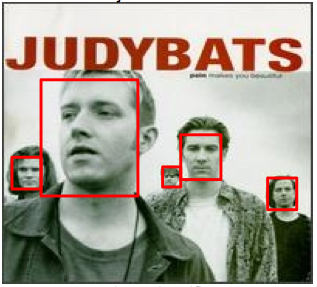
\includegraphics[scale=0.7]{figures/output_example_face_detection} 
\newline
\caption{Example of an output of face detection}
\label{output_example_face_detection}
\end{center} 
\end{figure}

\noindent But at a low level, the output is not anymore an annotated image. The object detector has a basic component that is something required to say if an instance of the object of interest is contained in a certain region or sub-region of the original image or not. This is what a binary classifier does \cite{DIN08}. For example, what a binary classifier does can look like in figure~\ref{output_example_face_detection_binary_classifier} \cite{DIN08}.
\newline

\begin{figure}[!h]
\begin{center}
\noindent 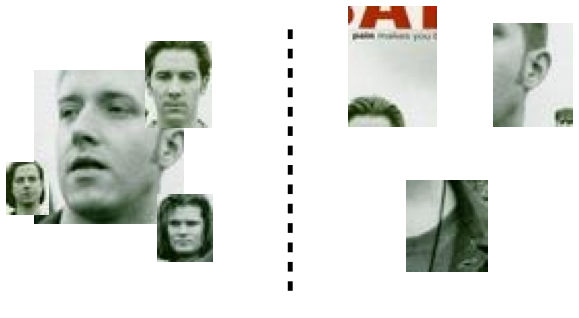
\includegraphics[scale=0.5]{figures/output_example_face_detection_binary_classifier} 
\newline
\caption{Example of what does a binary classifier for face detection}
\label{output_example_face_detection_binary_classifier}
\end{center} 
\end{figure}

\phantomsection
\section{Classifiers}

\vspace{\baselineskip}
\noindent Classification aim to solve the problem of identifying in a set of categories or sub-populations to which a new observation belongs. It is based on a training set of data that contains instances whose category affiliations are known. A classifier is an algorithm that implements classification. Classifiers groups data into categories. This can be done based on some measures of inherent similarity; for example, vectors represent the distance between instances, ad this in a multidimensional vector space \cite{CLASS}.
\newline










\newpage
\phantomsection
\chapter{Viola-Jones}

\noindent Viola-Jones algorithm is a visual object detection framework that is capable of processing images extremely rapidly while achieving high detection rates. It is based on a new image representation called "Integral Image" which allows the features used to be computed very quickly. It is also based on a learning algorithm, based on AdaBoost that gives extremely efficient classifiers. And it is also based on a method for combining classifiers in "cascade"; it allows to discard quickly the background of the image and to focus on the promising object-like regions \cite{VIO01}.
\newline

\phantomsection
\section{Haar features}

\noindent The features used by Viola and Jones are called Haar features and are based on Haar wavelets. Haar wavelets are single wavelength square waves (one high interval and one low interval). In two dimensions, a square wave is a pair of adjacent rectangles: one light and one dark. The actual rectangle combinations used for visual object detection are not true Haar wavelets. Instead, they contain rectangle combinations better suited to visual recognition tasks. That is because of this difference that these features are called Haar features, or Haarlike features, rather than Haar wavelets \cite{HEW07}.
\newline

\noindent For example, the figure~\ref{haar_features_first_2_stage} shows the first two Haar features in the original Viola-Jones cascade \cite{HEW07}. In the figure~\ref{haar_features_early_stage} , it is an example of a early stage in the Haar cascade. Each black and white patch represents a feature that the algorithm hunts for in the image \cite{HAR12}.
\newline

\begin{figure}[!h]
\begin{center}
\noindent 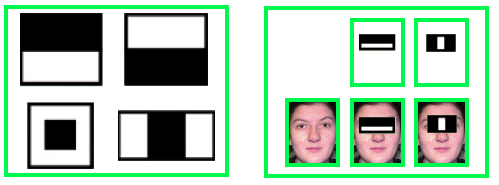
\includegraphics[scale=0.9]{figures/haar_features_first_2_stage} 
\newline
\caption{Example of the first two Haar features}
\label{haar_features_first_2_stage}
\end{center} 
\end{figure}

\begin{figure}[!h]
\begin{center}
\noindent 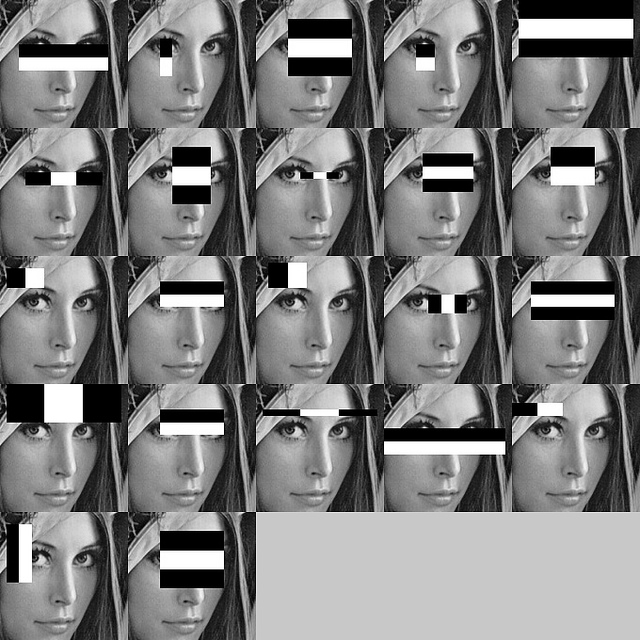
\includegraphics[scale=0.5]{figures/haar_features_early_stage} 
\newline
\caption{Example of an early stage in the Haar cascade}
\label{haar_features_early_stage}
\end{center} 
\end{figure}

\noindent The presence of a Haar feature is determined by subtracting the average dark-region pixel value from the average light-region pixel value. if the difference is above a threshold, that feature is said to be present and then it can go on to the next stage \cite{HEW07}. There is about 20-30 different stages. The first stage is a very coarse scan of the image. Stage 2 gets a little more detailed, stage 3 is a harder test to pass, stage 4 is even harder and it goes on and on. More it goes further into the cascade, more the features get increasingly complex and larger. It also takes more time to compute \cite{HAR12}.
\newline

\noindent For example, the figure~\ref{haar_feature_later_stage} shows the later stage in the Haar cascade where many more patterns of black and white rectangles need to match the candidate image \cite{HAR12}.
\newline

\begin{figure}[!h]
\begin{center}
\noindent 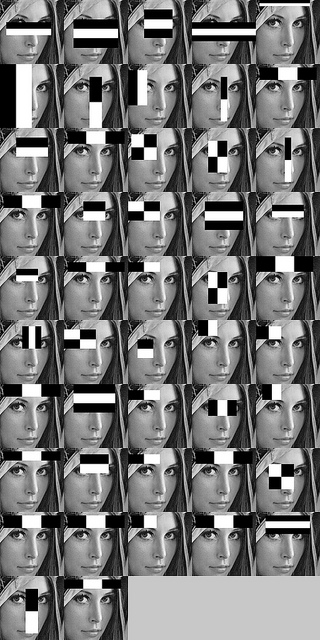
\includegraphics[scale=0.8]{figures/haar_feature_later_stage} 
\newline
\caption{Example of the later stage in the Haar cascade}
\label{haar_feature_later_stage}
\end{center} 
\end{figure}

\noindent Three kinds of feature are used by Viola and Jones. The value of a two-rectangle feature is the difference between the sum of the pixels within two rectangular regions. The regions have the same size and shape and are horizontally or vertically adjacent. A three-rectangle feature computes the sum within two outside rectangles subtracted from the sum in a center rectangle. Finally a four-rectangle feature computes the difference between diagonal pairs of rectangles \cite{VIO01}.
\newline

\noindent For example, the figure~\ref{haar_feature_description} shows the different kinds of rectangle features used by the Viola-Jones algorithm. Two-rectangle features are shown in (A) and (B). Figure (C) shows a three-rectangle feature, and (D) a four-rectangle feature \cite{VIO01}.
\newline

\begin{figure}[!h]
\begin{center}
\noindent 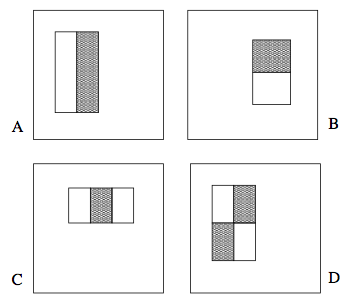
\includegraphics[scale=0.6]{figures/haar_feature_description} 
\newline
\caption{Example of the different kinds of rectangle features}
\label{haar_feature_description}
\end{center} 
\end{figure}

\phantomsection
\section{Integral image}

\noindent bla bla bla
\newline

\phantomsection
\section{Weak classifiers}

\noindent bla bla bla
\newline

\phantomsection
\section{AdaBoost}

\noindent bla bla bla
\newline

\phantomsection
\section{Test set and training}

\noindent bla bla bla
\newline

